\documentclass[ddcfooter]{tudbeamer}
\usepackage[utf8]{inputenc}
\usepackage{german}

\begin{document}
\title[Digital Signal Processing]{Digital Signal Processing using CUDA}
\subtitle{Digital Signal Processing using CUDA}
\author{Nico Wehmeyer, Richard Pfeifer, Fabian Jung}

\maketitle

\begin{frame}
    \frametitle*{Inhalt}
    \tableofcontents[currentsection]
\end{frame}

%Verantwortlicher: Richard
\section{Aufgabenstellung}
\begin{frame}
\frametitle{Aufgabenstellung}
%\framesubtitle{untertitel erste folie}
\begin{itemize} 
	\item{Ausgangsitutation}
	\begin{itemize}
		\item{Messgeräte erzeugen Datenstrom} %TODO(Nico) Datenbild
		\item{Datenstrom nicht kontinuierlich}
		\item{Serielle Implementierung}
	\end{itemize}
	\item{Anforderungen}
	\begin{itemize}
		\item{Portierung auf GPU}
		\item{Hoher Datendurchsatz}
		\item{Skalierbar auf bis zu 4 GPUs/Node}
	\end{itemize}
\end{itemize}
\end{frame}

%Verantwortlicher: Richard
\section{Überblick}
\begin{frame}
    \frametitle*{Überblick}
	\begin{itemize}
	\item{Host}
	\begin{itemize}
		%TODO
		\item{Eingabe Datei auslesen}
		\item{Daten zwischenspeichern}
	\end{itemize}
	\item{Levenberg Marquardt}
	\begin{itemize}
		%TODO
		\item{Parameter einer Näherungsfunktion bestimmen}
		\item{Markante Stellen (Anfangs-, Endwert, Maximum) ermitteln und zurückgeben}
	\end{itemize}
	\item{Verwaltung Devices}
	\begin{itemize}
		\item{Daten aus Puffer lesen}
		\item{Zu den Devices streamen}
		\item{Kernel starten}
		\item{Ausgabe schreiben}
	\end{itemize}
	\end{itemize}
\end{frame}
%Verantwortlicher: Richard
\section{Host Code}
\begin{frame}
    \frametitle*{Host: Lesen der Daten}
    \begin{minipage}{0.6\textwidth}
        \begin{figure}
            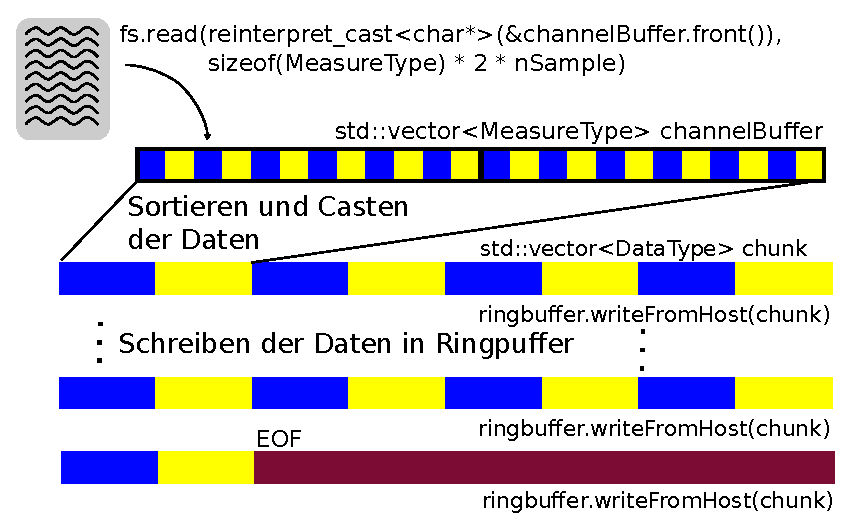
\includegraphics[scale=.5]{Datareader.eps}
        \end{figure}
    \end{minipage} \hfill
    \begin{minipage}{0.28\textwidth}
        \begin{itemize}
            \item Lesen von Daten zweier Kanäle
            \item Kanaltrennung
            \item Casten der Daten
            \item Sammeln mehrerer Signale zu Chunks
            \item Letzter Chunk wird mit Nullen gefüllt.
        \end{itemize}
    \end{minipage}
\end{frame}
\begin{frame}
    \frametitle*{Host: Ringpuffer}
    \begin{itemize}
        \item Messdatenfile $\rightarrow$ DataReader $\rightarrow$ Ringpuffer $\rightarrow$ GPU
        \item Speicher des Ringpuffer: Vektor dessen Typ per Template frei gewählt werden kann
        \item Host-GPU-Transfer wird wie folgt gelöst:
    \end{itemize}
    \begin{figure}
        \centering
        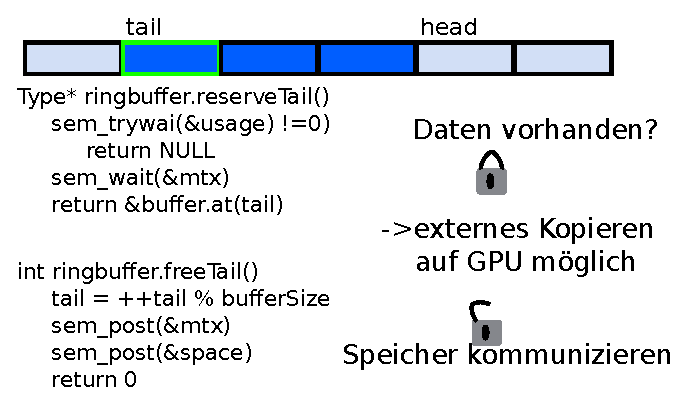
\includegraphics[scale=.5]{Ringbuffer.eps}
    \end{figure}
\end{frame}
\section{Levenberg Marquardt}
%Verantwortlicher: Nico
\begin{frame}
    \frametitle*{Levenberg Marquardt (1)}
    \begin{itemize}
        \item{Eingabedaten}
        	\begin{itemize}
        		\item{Samples}
	        		\begin{itemize}
	        			\item{Compute Capability 1.x: ca. 800)}
	        			\item{Compute Capability 2.0 oder höher: ca. 2500)}
	        		\end{itemize}
        		\item{Interpolationsschritt}
	        		\begin{itemize}
	        			\item{beliebige Dezimalzahl größer 0)}
	        			\item{Interpolation durch Texture Memory)}
	        		\end{itemize}
        	\end{itemize}
    \end{itemize}
\end{frame}
\begin{frame}
    \frametitle*{Levenberg Marquardt (2)}
    \begin{itemize}
        \item{Verarbeitung}
            \begin{itemize}
             	\item{eine Ausgleichungsrechnung pro Block}
             	\item{Grund: ca. das 5-fache der Sampleanzahl an Shared Memory benötigt (bei 1000 Samples ca. 20 kB)}
             	\item{Zugriff auf Samples durch Texture Memory}
	             	\begin{itemize}
	             	    \item{Shared Memory gespart}
	             	    \item{schnelle Interpolation möglich}
	             	\end{itemize}
             	\item{Vorgehensweise}
	             	\begin{itemize}
	           	        \item{Anfangs- und Endwert ermitteln}
	           	        \item{abhängig vom Schwellwert Bereich festlegen}
	           	        \item{für den Bereich Näherungsfunktion ermitteln}
	           	        \item{Qualität durch Residuen und Maximum der Funktion ermitteln}
	         	    \end{itemize}
            \end{itemize}
    \end{itemize}
\end{frame}
\begin{frame}
    \frametitle*{Levenberg Marquardt (3)}
	\begin{itemize}
        \item{Ausgabedaten}
        	\begin{itemize}
        		\item{3 Parameter einer quadratischen Funktion: $a*x^2+b*x+c$}
        		\item{Anfangs- und Endwert}
        		\item{Maximum}
        		\item{durchschnittliche Abweichung}
        		\item{Status (Fehler, Erfolg, Abbruch)}
        		
        	\end{itemize}
    \end{itemize}
\end{frame}
\begin{frame}
    \frametitle*{Levenberg Marquardt (4)}
	\begin{itemize}
        \item{Ergebnis: $fitfunktion=-0.550151*x^2+654.15509*x-203167.921875$}
        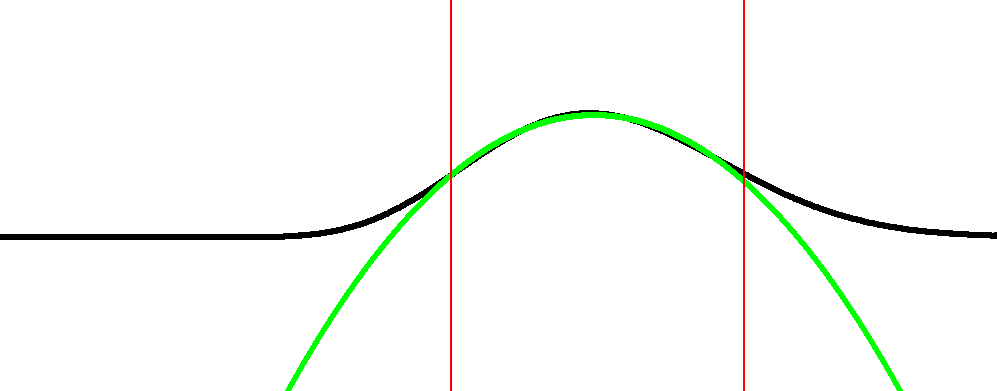
\includegraphics[height=3.5cm]{Beispielergebnis.png}
    \end{itemize}
\end{frame}
%Verantwortlicher: Fabian
\section{Verwaltung Devices}
\begin{frame}
    \frametitle*{Verwaltung Devices}
    \begin{itemize}
    	\item{Jedes Devices wird von einem Thread verwaltet}
    	\item{Asynchrone Aufrufe}
		\begin{itemize}
			\item{cudaMemcpyAsync}
			\item{Kernel}
			\item{Ermöglicht Pipeline}
		\end{itemize}
    	\item{Eigener Thread für Ausgabedatenstrom}
    \end{itemize}
\end{frame}

\section{Benchmark}
%Verantwortlicher: Fabian
\begin{frame}
    \frametitle*{Benchmark}
    \begin{center}
    \begin{tabular}{|r|r|r|r|r|}
    \hline
	GPUs & Datei    & Zeit     & Rate       & Normiert  \\
	\hline
	1    & 247MB	& 72.450s  &  3.41 MB/s & 3.41 MB/s \\
	2	 & 247MB	& 38.141s  &  6.48 MB/s & 3.24 MB/s \\
	3	 & 247MB	& 29.060s  &  8.50 MB/s & 2.83 MB/s \\
	4	 & 247MB	& 20.828s  & 11.85 MB/s & 2.96 MB/s \\
	1	 & 382MB	& 107.902s &  3.54 MB/s & 3.54 MB/s \\
	2	 & 382MB	& 57.537s  &  6.64 MB/s & 3.32 MB/s \\
	3	 & 382MB	& 40.951s  &  9.33 MB/s & 3.11 MB/s \\
	4	 & 382MB	& 29.885s  & 12.78 MB/s & 3.20 MB/s \\
	\hline
	\end{tabular}
	\end{center}
\end{frame}
\section{Skalierbarkeit}
%Verantwortlicher: ???
\begin{frame}
    \frametitle*{Skalierbarkeit}
    \begin{itemize}
        \item{Horizontal Skalierbar}
        \item{PCIe Bus noch nicht vollständig ausgelastet}
        \item{Reserven in der Implementierung des Ringbuffers}
    \end{itemize}

\end{frame}
\section{Danksagung}

\begin{frame}
    \frametitle*{Danksagung}
    %TODO: Sinnvollere Satzbildung

    \begin{block} ~
    \begin{center}
    Vielen Dank an \\Dr. Michael Bussmann, Axel Hübel und Rene Widera \\ für Diskussion und Optimierungsvorschläge.
    \end{center}
    \end{block}

\end{frame}
\end{document}
